
\documentclass[10pt, a4paper]{article}
\usepackage[a4paper,outer=1.5cm,inner=1.5cm,top=1.75cm,bottom=1.5cm]{geometry}

\twocolumn
\usepackage{graphicx}
\usepackage{karnaugh-map}
\usepackage{tabularx}
\usepackage{hyperref}
\usepackage[utf8]{inputenc}
\usepackage{amsmath}
\usepackage{physics}
\usepackage{amssymb}
\usepackage{listings}
\providecommand{\norm}[1]{\left\lVert#1\right\rVert}
\providecommand{\abs}[1]{\left\vert#1\right\vert}
\let\vec\mathbf
\newcommand{\myvec}[1]{\ensuremath{\begin{pmatrix}#1\end{pmatrix}}}
\newcommand{\mydet}[1]{\ensuremath{\begin{vmatrix}#1\end{vmatrix}}}
\providecommand{\brak}[1]{\ensuremath{\left(#1\right)}}
\begin{document}
\title{Optimization Assignment}
\author{Name:Soundarya Naru\and Email :  \url{narusoundarya2002@gmail.com.com}}
%\{ Wireless Communication (FWC)}
\date{}
\maketitle
  \section{Problem}
A merchant plans to sell two types
of personal computers a desktop model and a portable
model that will cost Rs 25000 and Rs 40000 respectively. He
estimates that the total monthly demand of computers will
not exceed 250 units. Determine the number of units of each
type of computers which the merchant should stock to get
maximum profit if he does not want to invest more than Rs
70 lakhs and if his profit on the desktop model is Rs 4500
and on portable model is Rs 5000.
\section{Solution}
Let's assume that
\begin{center}
Number of Desktops be x\\
Number of Portable computers be y\\
\end{center}
\begin{tabular}{|c|c|c|c|}
	\hline
	\textbf{Item}&\textbf{Number}&\textbf{Cost}&\textbf{Profit}\\
	\hline
	Desktop&x&25000&4500\\
	\hline
	Portable Computers&y&40000&5000\\
	\hline
	Max Investment& &7000000&\\
	\hline
\end{tabular}\\
According to question:\\
Monthly demand of both items=Maximum 250 units\\
\begin{align}
\myvec{1&1}\myvec{x\\y} \le 250 
\end{align}
Also,\\
\begin{center}
	cost of Desktop=$Rs.2500$\\
	cost of computers=$Rs.40000$\\
	Maximum investment=$Rs.7000000$\\
\end{center}
Hence,
\begin{align}
 \myvec{25000&40000}\myvec{x\\y} \le 7000000 \\
=>\myvec{5&8}\myvec{x\\y} \le 1400 
\end{align}
\begin{center}
 As we need to maximize profit,\\
Hence,function used here will be maximize Z\\
	profit on Desktop=$Rs.4500$\\
	profit on computers=$Rs.5000$\\
	$\therefore$ maximize Z=$\myvec{4500&5000}\myvec{x\\y}$\\ 
\end{center}
combining all constraints
\begin{center}
	Maximize Z=$\myvec{4500&5000}\myvec{x\\y}$\\
	subject to constraints\\
\end{center}
\begin{align}
 \myvec{1&1\\5&8}\myvec{x\\y} \le \myvec{250\\1400} \\
 x \geq 0,y \geq 0
\end{align}
\begin{align}
 \myvec{1&1}\myvec{x\\y} \le 250 
\end{align}
\begin{center}
\begin{tabular}{|c|c|c|}
	\hline
	x&0&250\\
	\hline
	y&250&0\\
	\hline
\end{tabular}\\
\end{center}
\begin{align}
 \myvec{5&8}\myvec{x\\y} \le 1400 
\end{align}
\begin{center}
\begin{tabular}{|c|c|c|}
	\hline
	x&280&0\\
	\hline
	y&0&175\\
	\hline
\end{tabular}\\
\end{center}
\begin{center}
\begin{tabular}{|c|c|}
	\hline
	\textbf{Corner points}&\textbf{Value of Z}\\
	\hline
	(250,0)&112500\\
    \hline
	(200,50)&1150000\\
	\hline
	(0,175)&875000\\
	\hline
\end{tabular}\\
\end{center}
\begin{center}
Hence,the profit will be maximum if company produces\\
	Number of Desktops is 200\\
	Number of Portable computers is 50\\
	Maximum profit is 1150000\\
\end{center}
\section{Construction}
\begin{figure}[h]
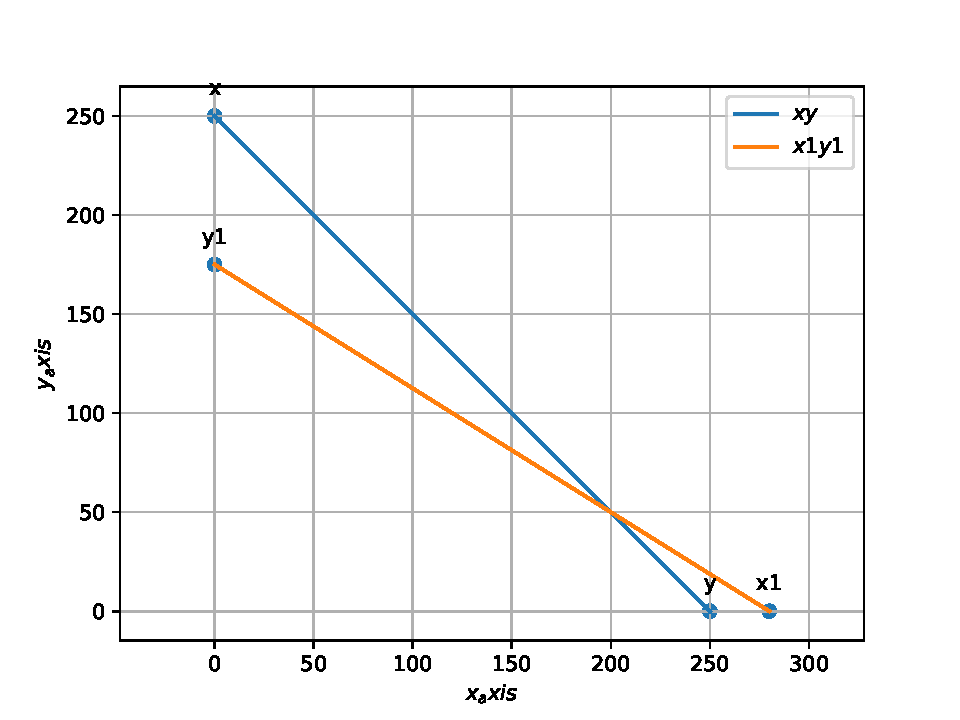
\includegraphics[scale=0.5]{opti_1.pdf} 
\end{figure}
\section{Execution}
Verify the above proofs in the following code.\\
\begin{lstlisting}
https://github.com/soundaryanaru/FWC-assignments/blob/main/Optimization/Basic/code/op.py
\end{lstlisting}
 \bibliographystyle{ieeetr}
\end{document}
